% 独自のコマンド

% ■ アブストラクト
%	\begin{jabstract} 〜 \end{jabstract}	:日本語のアブストラクト
%	\begin{eabstract} 〜 \end{eabstract}	:英語のアブストラクト

% ■ 謝辞
%	\begin{acknowledgment} 〜 \end{acknowledgment}

% ■ 文献リスト
%	\begin{bib}[100] 〜 \end{bib}

\newif\ifjapanese
\newif\ifjabstructtitledifferent
\japanesetrue
\jabstructtitledifferenttrue

\ifjapanese
	\documentclass[11pt, dvipdfmx]{jreport}
	\renewcommand{\bibname}{参考文献}
	\newcommand{\acknowledgmentname}{謝辞}
\else
	\documentclass[11pt, dvipdfmx]{report}
	\newcommand{\acknowledgmentname}{Acknowledgment}
\fi

\usepackage{docmute}
% 各ファイル共通の設定を記述
\usepackage{ascmac}
\usepackage{graphicx}
\usepackage{multirow}
\usepackage{url}
\usepackage{otf} %髙橋先生の”髙”
\usepackage[setpagesize=false]{hyperref}
\usepackage{pxjahyper}
\usepackage{subcaption}
\usepackage{ylab_thesis}

\makeatletter

\newcommand\myprintindex{	% 索引を目次に追加
	\clearpage
	\phantomsection
	\addcontentsline{toc}{chapter}{\indexname}
	\printindex
}

\makeatother



%\bindermode	% バインダ用余白設定

% 日本語情報
\jclass {卒業論文}
\jtitle {hogeに関する検討}
\jabstructtitle{非線形メトリック最適化によるネットワークの \\ 信頼性向上法に関する研究}
\juniv {秋田大学 \ 理工学部}
\jfaculty {数理・電気電子情報学科 \ 人間情報工学コース}
\jauthor {1234567 \ hoge下 \ hoge夫}
\jadvisor {橋本 \ 仁 \ 准教授}
\jhyear{29}
\jsyear {2017}
\jkeyword{hoge, hoge, hoge} 

\begin{document}

\jmaketitle	% 表紙(日本語)

\begin{jabstract}

hogeを検討するよ

\end{jabstract}


\tableofcontents	% 目次
\listoffigures	% 表目次
\listoftables		% 図目次

\pagenumbering{arabic}

% 第1章
\documentclass[11pt, dvipdfmx]{jreport}

% 各ファイル共通の設定を記述
\usepackage{ascmac}
\usepackage{graphicx}
\usepackage{multirow}
\usepackage{url}
\usepackage{otf} %髙橋先生の”髙”
\usepackage[setpagesize=false]{hyperref}
\usepackage{pxjahyper}
\usepackage{subcaption}
\usepackage{ylab_thesis}

\makeatletter

\newcommand\myprintindex{	% 索引を目次に追加
	\clearpage
	\phantomsection
	\addcontentsline{toc}{chapter}{\indexname}
	\printindex
}

\makeatother



\begin{document}

\chapter{序論}
\label{chap:Introduction}

\section{研究背景}

俺達は雰囲気でTeXをやっている.

\section{研究目的}

\section{本論文の構成}

\end{document}

% 第2章
\documentclass[11pt, dvipdfmx]{jreport}

% 各ファイル共通の設定を記述
\usepackage{ascmac}
\usepackage{graphicx}
\usepackage{multirow}
\usepackage{url}
\usepackage{otf} %髙橋先生の”髙”
\usepackage[setpagesize=false]{hyperref}
\usepackage{pxjahyper}
\usepackage{subcaption}
\usepackage{ylab_thesis}

\makeatletter

\newcommand\myprintindex{	% 索引を目次に追加
	\clearpage
	\phantomsection
	\addcontentsline{toc}{chapter}{\indexname}
	\printindex
}

\makeatother



\begin{document}
% 分割ファイル,メインファイルから画像フォルダへの相対パスを記述する
\graphicspath{{../figure/}{./figure/}}

\chapter{hoge}
\label{chap:hoge}

\section{aaa}

図の例を示します.

\begin{figure}[htbp]
  \begin{center}
    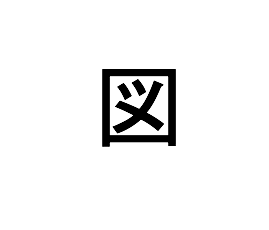
\includegraphics{figure_example.png}
    \caption{図}
    \label{fig:figure_example}
  \end{center}
\end{figure}

\section{bbb}

表の例を示します.

\begin{table}[htb]
  \begin{center}
    \caption{表}
    \begin{tabular}{|c|c|c|} \hline
      県名 & かな & ローマ字 \\ \hline \hline
      秋田 & あきた & Akita \\
      東京 & とうきょう & Tokyo \\
      吉田 & よしだ & Yoshida \\ \hline
    \end{tabular}
    \label{tab:prefecture}
  \end{center}
\end{table}

\section{ccc}

\section{ddd}

\section{eee}

\end{document}

% 第3章
\documentclass[11pt, dvipdfmx]{jreport}

% 各ファイル共通の設定を記述
\usepackage{ascmac}
\usepackage{graphicx}
\usepackage{multirow}
\usepackage{url}
\usepackage{otf} %髙橋先生の”髙”
\usepackage[setpagesize=false]{hyperref}
\usepackage{pxjahyper}
\usepackage{subcaption}
\usepackage{ylab_thesis}

\makeatletter

\newcommand\myprintindex{	% 索引を目次に追加
	\clearpage
	\phantomsection
	\addcontentsline{toc}{chapter}{\indexname}
	\printindex
}

\makeatother



\begin{document}

\chapter{hogehoge}
\label{chap:hogehoge}

\section{aaa}

\section{bbb}

\section{ccc}

\section{ddd}

\end{document}

%第4章

\chapter{hogehogehoge}
\label{chap:hogehogehoge}

%第5章

\chapter{hogehogehogehoge}
\label{chap:hogehogehogehoge}


\input{parts/90_Acknowledgment} % 謝辞
% 参考文献

\begin{thebibliography}{99}
	\bibitem{OSPF}
	J.T.Moy: OSPF version 2, IETF, 
	RFC 2328, \url{http://search.ietf.org/rfc/rfc2328.txt}, April 1998
	
	\bibitem{multi-topology}
	“Multi-Topology(MT) Routing in OSPF”, RFC4915, Jun., 2009.
	
	\bibitem{cost239}
	O’Mahony, M., Sinclair, M.C., and Mirac, B. : Ultra high Capacity Optical Transmission Network : European
	Reserch, Project COST 239, Information, Telecommunications, Automata Journal, vol.12, pp.33-46, June
	1993.

	\bibitem{nsfnet}
	Niu, X., Zhong, W.D., Shen, G. and Cheng, T.H. : Connection Establishment of Label Switched Paths in
	IP/MPLS over Opticak Networks, Photnic Network Communications, vol.6, pp.33-41, July 2003.
	
	
\end{thebibliography}

\end{document}
